\section{Auswertung}
\label{sec:Auswertung}

\subsection{Fouriesynthese}
Im ersten Teil des Experiments wurden wie in der Durchführung beschrieben die Spannungsverläufe zusammengesetzt. 

In Abbildung (\ref{fig:plot1}) ist die Fouriereihe der Sägezahnspannung zu sehen.
\begin{figure}[H]
  \centering
  \includegraphics[width = 0.7\linewidth]{Sägezahn.jpeg}
  \caption{Verlauf der Sägezahnspannung.}
  \label{fig:plot1}
\end{figure}

In Abbildung (\ref{fig:plot2}) ist die Fouriereihe der Dreiecksspannung zu erkennen. 
\begin{figure}[H]
  \centering
  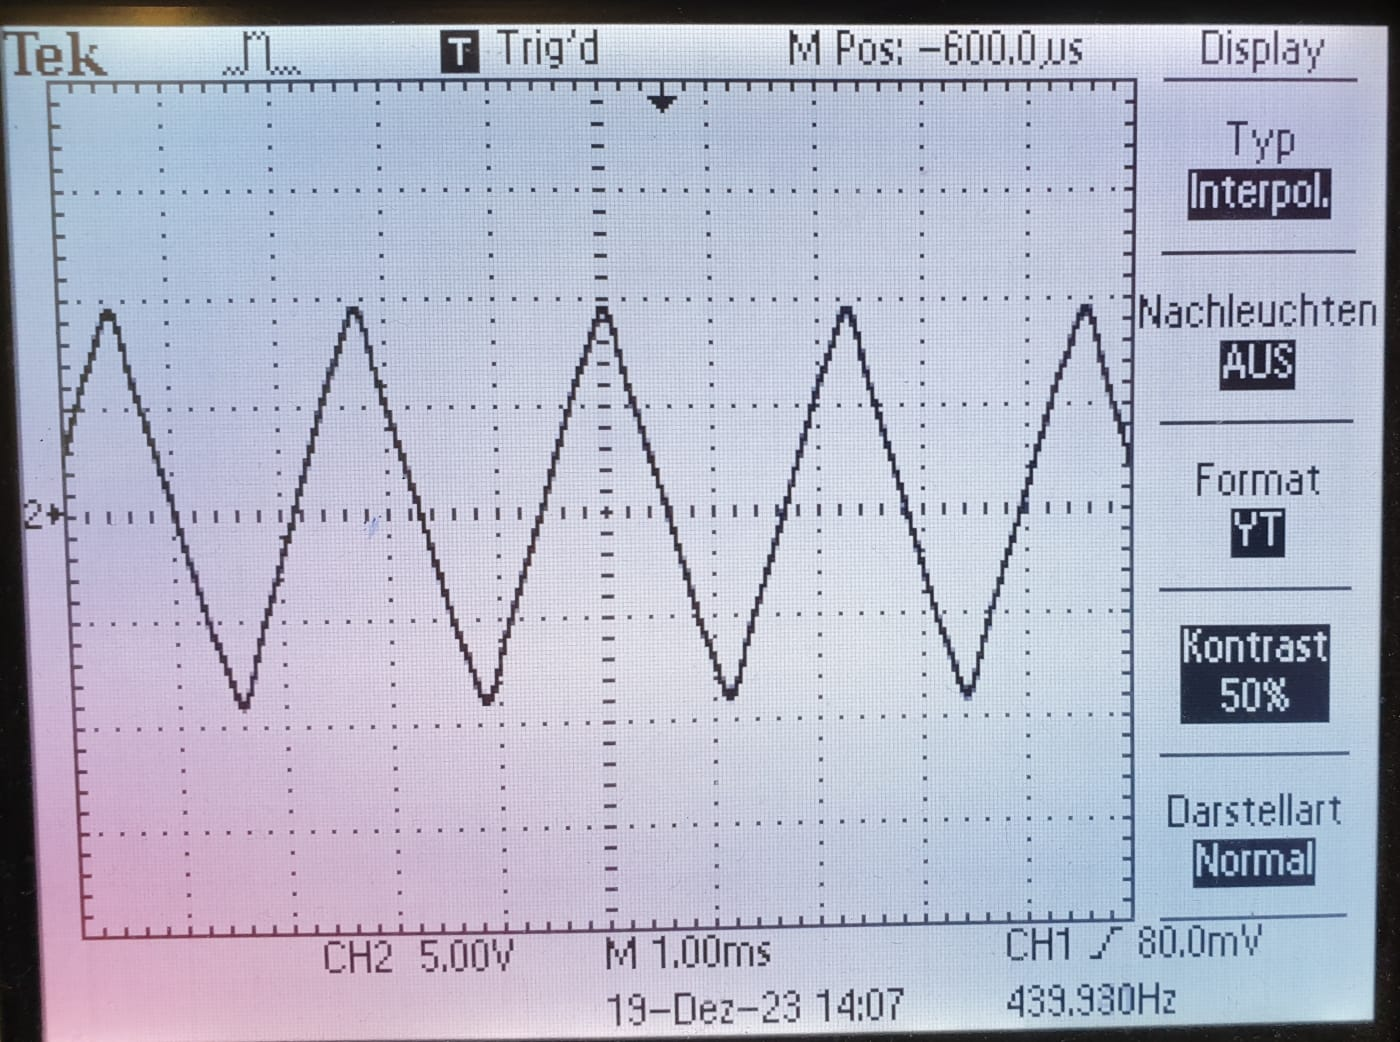
\includegraphics[width = 0.7\linewidth]{Dreieck.jpeg}
  \caption{Verlauf der Dreiecksspannung.}
  \label{fig:plot2}
\end{figure}

Außerdem ist in Abbildung (\ref{fig:plot3}) die Fouriereihe der Rechteckspannung
\begin{figure}[H]
  \centering
  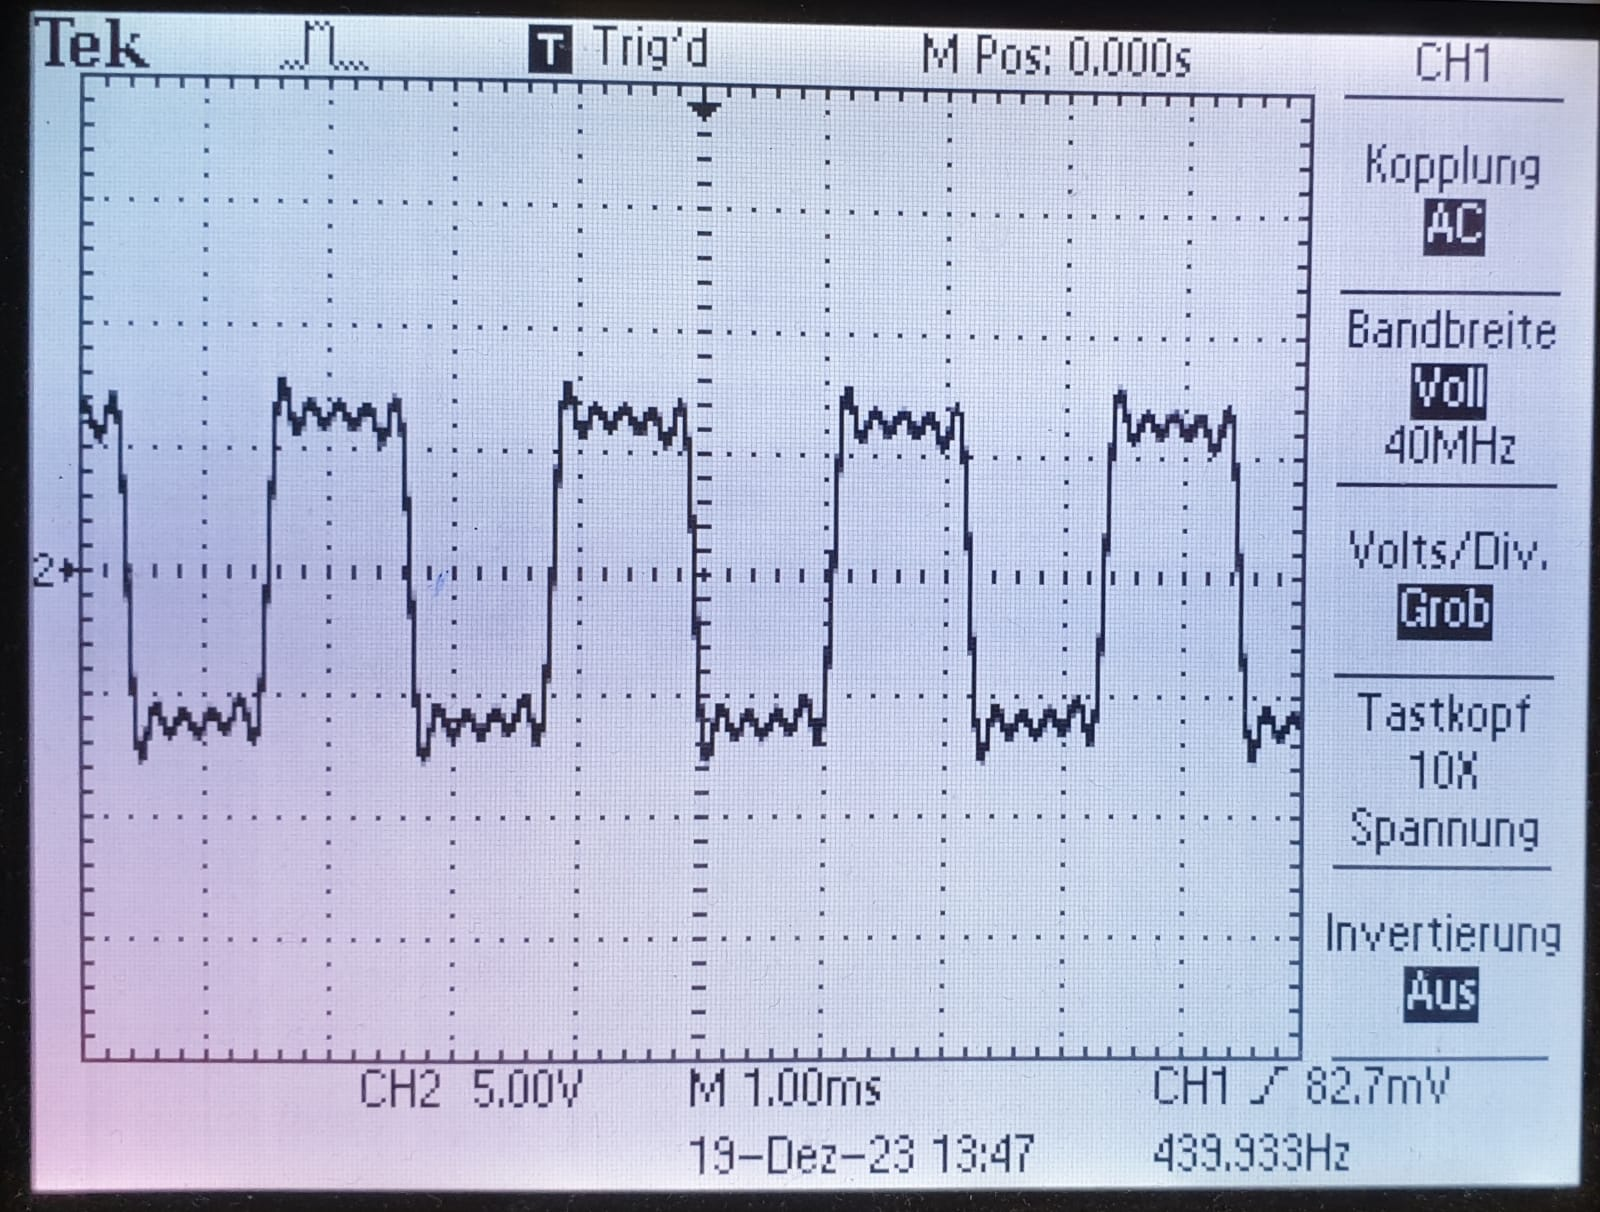
\includegraphics[width = 0.7\linewidth]{Viereck.jpeg}
  \caption{Verlauf der Rechteckspannung.}
  \label{fig:plot2}
\end{figure}

\subsection{Fourieanalyse}
Im zweiten Teil des Experiments wurde das Linienspektrums der Sägezahnspannung, Dreiecksspannung und Rechteckspannung auf dem Oszilloskop eingestellt, um dann 
mithilfe des Cursers die Höhe der Peaks messen zu können. \\
\\
\textbf{Sägezahnspannung} \\
Die Frequenz wird in Kilohertz und die Höhe der Peaks wird in Dezibil gemessen. Die aufgenommenen Messdaten sind in Tabelle (\ref{tab:saegezahn}) aufgeführt. 
\begin{table}[H]
  \centering
  \caption{Gemessene Spannung in Abhängigkeit der Frequenz.}
  \label{tab:saegezahn}
  \begin{tblr}{colspec={c c}}
      \toprule
      $f\,[\unit{\kilo\hertz}]$ & $U\,[\unit{\decibel}]$ \\
      \midrule
      10 & 33,0 \\
      20 & 27,0 \\
      30 & 23,4 \\
      40 & 21,0 \\
      50 & 19,0 \\
      60 & 17,4 \\
      70 & 16,2 \\
      80 & 14,6 \\
      90 & 13,4 \\
      100 & 13,0 \\
      110 & 12,2 \\
      \bottomrule
  \end{tblr}
\end{table}
Die Amplitude wird zur weiteren Betrachtung der Daten von Dezibil in Volt umgerechnet durch 
$$\unit{\volt} \sim  10 ^{\frac{\unit{\decibel}}{20}} \, .$$
Diese Messwerte werden in Abbildung (\ref{fig:saeg}) aufgetragen. Zusätzlich wird eine Ausgleichsfunktion berechnet, die durch
$$ U(x) = \symup{a} \cdot x^{\symup{b}} $$
definiert ist. 
Für die Sägezahnspannung wurden die Werte 
\begin{align*}
  \symup{a}_1 &= (451 \pm 4) \cdot 10^{-3} \, \unit{\volt\second} \\
  \symup{b}_1 &= -1,0036 \pm 0,0035
\end{align*}
%\\
\textbf{Dreiecksspannung} \\

\textbf{Rechteckspannung} \\




%a_saeg: 450.68807906140404, b_saeg: -1.0035509703352652
%a = 450.6881 ± 4.3789
%b = -1.0036 ± 0.0035
%a_recht: 877.8485996440896, b_recht: -0.993873520862041
%c = 877.8486 ± 5.1405
%d = -0.9939 ± 0.0022
%a_drei: 5381.273099208562, b_drei: -1.9808594085522564
%e = 5381.2731 ± 90.5629
%f = -1.9809 ± 0.0072


%Siehe \autoref{fig:plot}!